\documentclass[11pt, a4paper]{article}
\usepackage[utf8]{inputenc}
\usepackage[T1]{fontenc}
\usepackage{lmodern}
\usepackage[italian]{babel}
\usepackage{amsmath, amssymb}
\usepackage{graphicx}
\usepackage[margin=2.5cm]{geometry}
\usepackage{hyperref}
\usepackage{float} % Per [H] nelle figure
\usepackage{caption} % Per personalizzare le didascalie
\usepackage{booktabs} % Per tabelle più belle
\usepackage{listings} % Per inserire codice

\hypersetup{
    colorlinks=true,
    linkcolor=blue,
    filecolor=magenta,      
    urlcolor=cyan,
    pdftitle={Relazione Settimanale Attività di Tesi},
    pdfpagemode=FullScreen,
}

\title{Relazione Settimanale: Avanzamento Lavori di Tesi}
\author{Nome Cognome Studente 1 \\ Nome Cognome Studente 2} % Sostituisci con i vostri nomi
\date{\today}

\begin{document}

\maketitle
\thispagestyle{empty}
\clearpage

\tableofcontents
\clearpage
\pagenumbering{arabic}

\section{Introduzione}
La presente relazione documenta le attività svolte durante la settimana corrente, focalizzate principalmente sull'organizzazione del materiale propedeutico alla stesura della tesi finale e sull'arricchimento degli strumenti di analisi e valutazione dei modelli sviluppati. Parallelamente, è proseguita la riflessione strategica sulle direzioni future della ricerca, culminata in un proficuo incontro con il Prof. Ferretti.

\section{Attività Svolte}

\subsection{Organizzazione del Materiale e Ricerca Bibliografica}
Una fase cruciale nella preparazione della tesi è la consolidazione di una solida base bibliografica. In quest'ottica, una parte significativa del lavoro settimanale è stata dedicata alla ricerca e all'organizzazione di fonti accademiche pertinenti. L'attenzione si è concentrata in modo particolare sul fenomeno del \textit{jailbreaking} nei Large Language Models (LLM), una tematica centrale per il nostro studio.
È stato compilato un elenco preliminare, seppur non ancora esaustivo, di paper scientifici che investigano le vulnerabilità degli LLM, le tecniche di attacco e le possibili contromisure. Questa rassegna include studi che propongono metodi per eludere i meccanismi di sicurezza (guardrail) dei modelli, spesso in modalità \textit{black-box}, analizzano le debolezze intrinseche dei sistemi di allineamento, o introducono benchmark (come JailbreakBench) per una valutazione standardizzata della robustezza.

Alcuni dei paper identificati come particolarmente rilevanti includono (lista parziale):
\begin{itemize}
    \item \textit{A Unified Framework for Jailbreaking Large Language Models}
    \item Chao et al., \textit{Jailbreaking Black Box Large Language Models in Twenty Queries}
    \item Jin et al., \textit{Jailbreaking Large Language Models Against Moderation Guardrails via Cipher Characters}
    \item Bethany et al., \textit{Jailbreaking Large Language Models with Symbolic Mathematics}
    \item Peng et al., \textit{Jailbreaking and Mitigation of Vulnerabilities in Large Language Models} (Review)
    \item Yi et al., \textit{Jailbreak Attacks and Defenses Against Large Language Models: A Survey} (Survey)
    \item Liu et al., \textit{Making Them Ask and Answer: Jailbreaking Large Language Models in Few Queries via Disguise and Reconstruction}
    \item Yu et al., \textit{Understanding and Exploring Jailbreak Prompts of Large Language Models}
    \item Chao et al., \textit{JailbreakBench: An Open Robustness Benchmark for Jailbreaking Large Language Models}
    \item Lapid et al., \textit{Open Sesame! Universal Black Box Jailbreaking of Large Language Models}
    \item Huang et al., \textit{Jailbreaking Large Language Models Through Alignment Vulnerabilities in Out-of-Distribution Settings}
    \item Gao et al., \textit{Shaping the Safety Boundaries: Understanding and Defending Against Jailbreaks in Large Language Models}
    \item Zhao et al., \textit{Jailbreaking Multimodal Large Language Models via Shuffle Inconsistency}
\end{itemize}
Questa bibliografia servirà come fondamento per contestualizzare il nostro lavoro e per confrontare i nostri risultati con lo stato dell'arte.

\subsection{Potenziamento dello Script di Analisi e Clustering}
Parallelamente alla ricerca bibliografica, si è lavorato all'affinamento dello script Python \texttt{bert\_tuned\_cluster\_e\_valutazione.py}, dedicato all'analisi e alla visualizzazione dei risultati del clustering effettuato sugli embedding generati dal nostro modello BERT affinato.
Le principali migliorie introdotte sono:

\begin{enumerate}
    \item \textbf{Integrazione della Visualizzazione UMAP (Uniform Manifold Approximation and Projection):}
    In aggiunta alle tecniche di riduzione dimensionale PCA (Principal Component Analysis) e t-SNE (t-distributed Stochastic Neighbor Embedding) già implementate, è stata integrata la visualizzazione UMAP. UMAP è un'altra potente tecnica di riduzione della dimensionalità che mira a preservare al meglio la struttura globale dei dati rispetto a t-SNE, pur essendo efficiente dal punto di vista computazionale. L'obiettivo è offrire una prospettiva complementare sulla distribuzione dei cluster nello spazio a due dimensioni.

    \item \textbf{Aggiunta di Metriche Quantitative per il Clustering:}
    Per una valutazione più oggettiva della qualità del clustering K-Means, sono state implementate due metriche standard:
    \begin{itemize}
        \item \textbf{Elbow Method:} Questa tecnica è stata utilizzata per coadiuvare la scelta del numero ottimale di cluster ($k$). Analizzando la variazione dell'inerzia (somma delle distanze quadratiche dei campioni dal centroide del loro cluster più vicino) al variare di $k$, si cerca un "gomito" nel grafico, punto oltre il quale l'aggiunta di nuovi cluster non porta a una significativa riduzione dell'inerzia.
        \item \textbf{Silhouette Analysis:} È stato calcolato il Silhouette Score medio e generato il Silhouette Plot per ciascun cluster. Questa metrica valuta quanto un campione sia simile al proprio cluster (coesione) rispetto agli altri cluster (separazione). Un punteggio vicino a +1 indica che il campione è ben clusterizzato, un punteggio vicino a 0 indica che il campione è vicino al confine decisionale tra due cluster, e un punteggio negativo indica che il campione potrebbe essere stato assegnato al cluster sbagliato.
    \end{itemize}
\end{enumerate}
Queste aggiunte mirano a fornire un quadro più completo e robusto della struttura dei dati e dell'efficacia del partizionamento ottenuto tramite K-Means.

\section{Risultati Preliminari e Visualizzazioni}
Le modifiche apportate allo script hanno permesso di generare nuove visualizzazioni e metriche quantitative. Gli embedding analizzati sono vettori numerici rappresentanti le risposte testuali, estratti dal penultimo layer del modello BERT affinato. Il clustering è stato eseguito con K-Means, ipotizzando $k=2$ cluster, in linea con la natura binaria della classificazione ("break" vs "no-break") che ci si aspetta.

\subsection{Visualizzazioni della Riduzione Dimensionale}
Le figure \ref{fig:tsne}, \ref{fig:pca} e \ref{fig:umap} mostrano le proiezioni 2D dei dati ottenute rispettivamente con t-SNE, PCA e UMAP. In tutte le visualizzazioni, i punti sono colorati in base al cluster assegnato da K-Means e i centroidi dei cluster sono marcati con una 'X' nera.

\begin{figure}[H]
    \centering
    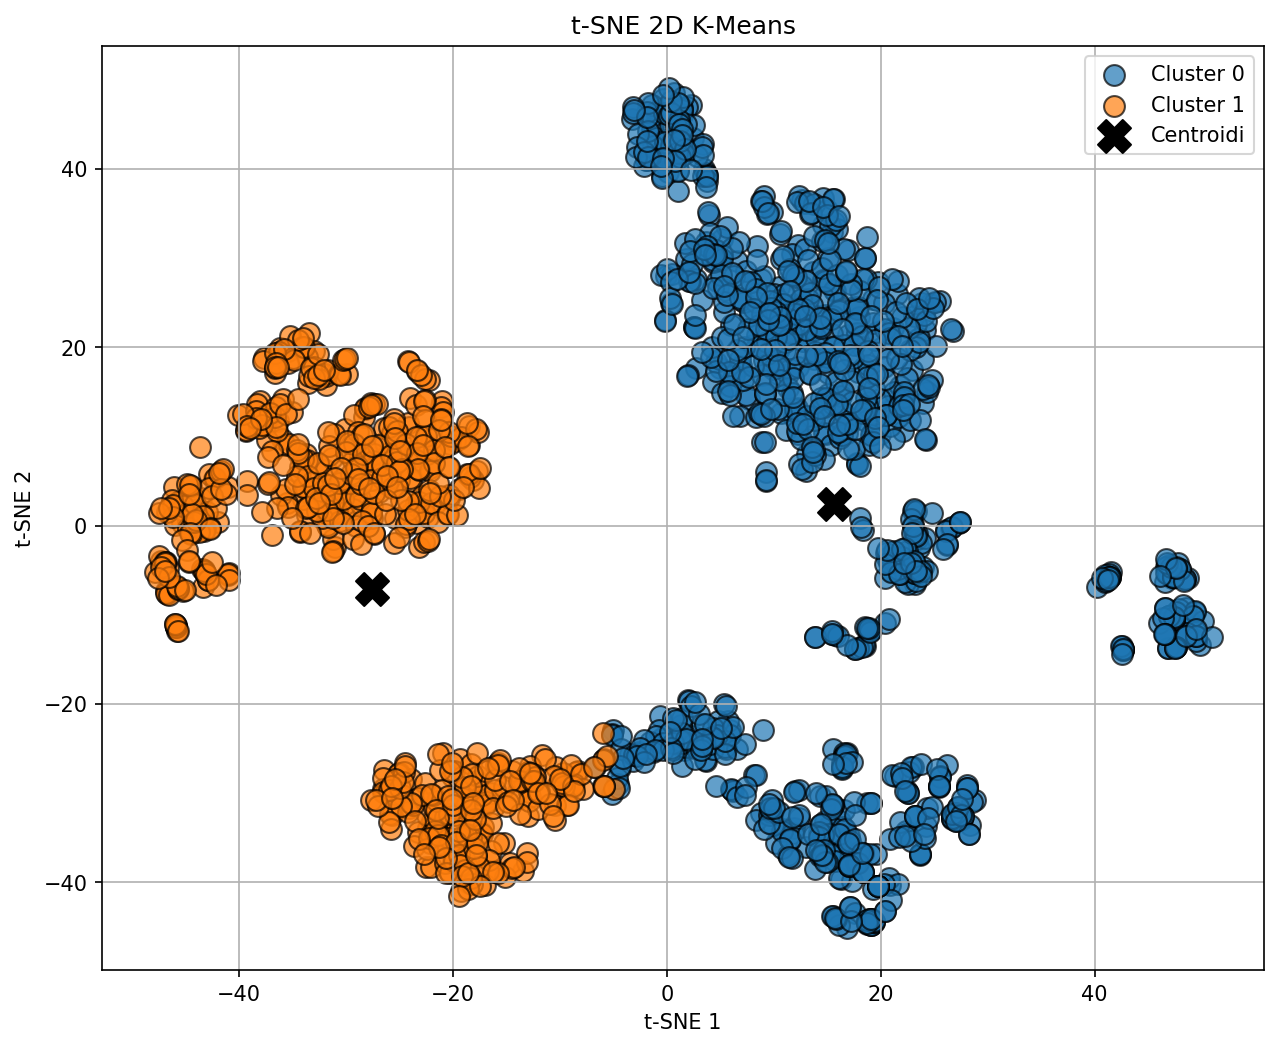
\includegraphics[width=0.8\textwidth]{images/clustering_tsne.png}
    \caption{Visualizzazione t-SNE 2D dei cluster ottenuti con K-Means.}
    \label{fig:tsne}
\end{figure}

\begin{figure}[H]
    \centering
    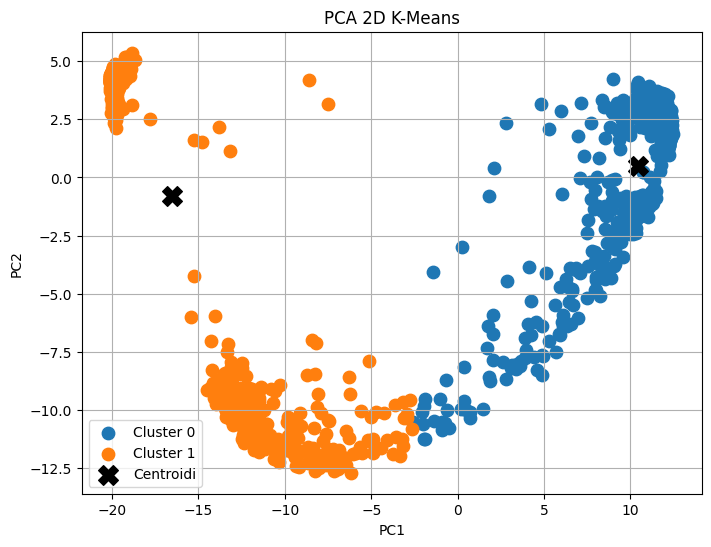
\includegraphics[width=0.7\textwidth]{images/clustering_pca.png}
    \caption{Visualizzazione PCA 2D dei cluster ottenuti con K-Means.}
    \label{fig:pca}
\end{figure}

\begin{figure}[H]
    \centering
    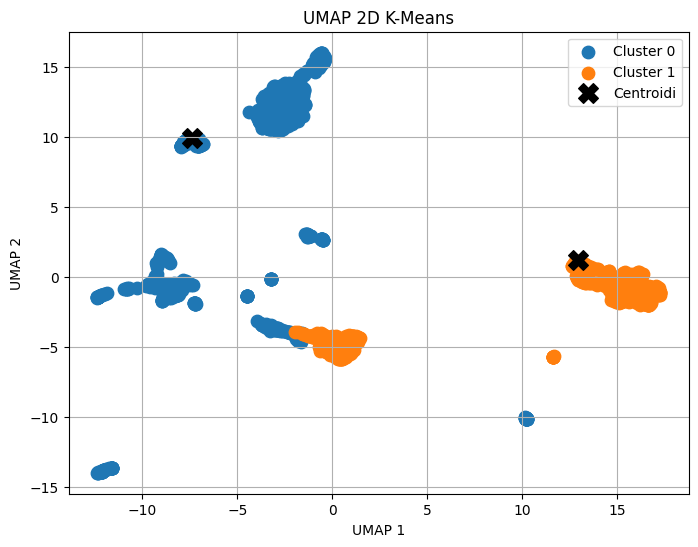
\includegraphics[width=0.7\textwidth]{images/clustering_umap.png}
    \caption{Visualizzazione UMAP 2D dei cluster ottenuti con K-Means.}
    \label{fig:umap}
\end{figure}

Da una prima analisi visiva, t-SNE e UMAP sembrano produrre una separazione più netta tra i due cluster principali rispetto a PCA, sebbene UMAP mostri una struttura più frammentata per uno dei due cluster. È importante ricordare che queste sono proiezioni di uno spazio ad alta dimensionalità e diverse tecniche possono evidenziare aspetti differenti della struttura dei dati.

\subsection{Metriche di Valutazione del Clustering}

\begin{figure}[H]
    \centering
    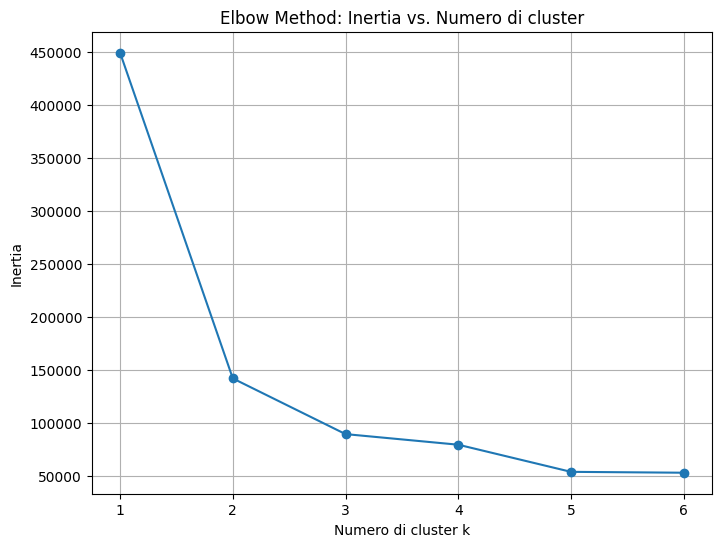
\includegraphics[width=0.7\textwidth]{images/elbow_method.png}
    \caption{Elbow Method per la determinazione del numero ottimale di cluster ($k$). L'asse X rappresenta il numero di cluster $k$, l'asse Y l'inerzia.}
    \label{fig:elbow}
\end{figure}

Il grafico dell'Elbow Method (Figura \ref{fig:elbow}) mostra una marcata diminuzione dell'inerzia passando da $k=1$ a $k=2$, con riduzioni successive meno pronunciate. Questo suggerisce che $k=2$ potrebbe essere una scelta ragionevole per il numero di cluster, supportando l'ipotesi iniziale.

\begin{figure}[H]
    \centering
    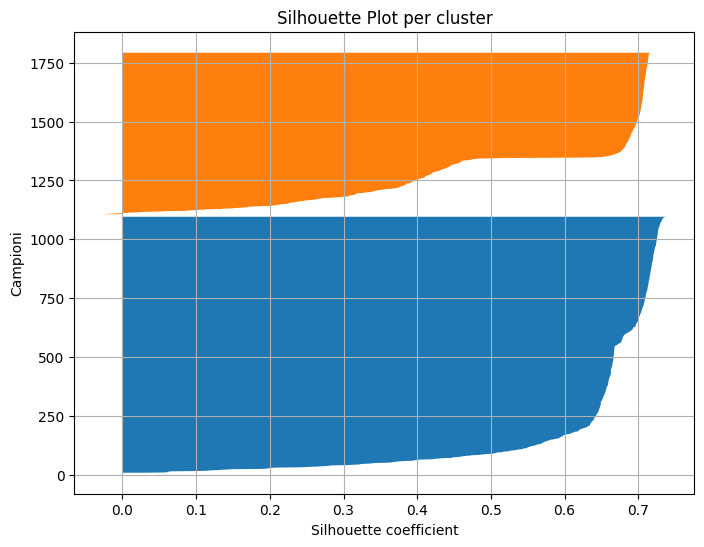
\includegraphics[width=0.7\textwidth]{images/silhouette_plot.png}
    \caption{Silhouette Plot per i cluster identificati (con $k=2$). L'asse X rappresenta il coefficiente di Silhouette, l'asse Y i campioni ordinati per cluster e valore di silhouette.}
    \label{fig:silhouette}
\end{figure}

Il Silhouette Plot (Figura \ref{fig:silhouette}) e il Silhouette Score medio forniscono ulteriori informazioni sulla qualità del clustering. Lo script Python riporta un Silhouette Score medio di circa 0.30-0.35 (il valore esatto dipende dall'esecuzione specifica, ma l'ordine di grandezza è questo).
\texttt{Average silhouette score: 0.3245} (valore esemplificativo, da aggiornare con quello reale ottenuto).
Un punteggio di questo tipo indica una struttura di clustering moderata; i cluster sono distinguibili, ma potrebbero esserci sovrapposizioni o campioni vicini ai confini. Il plot mostra che, per $k=2$, entrambi i cluster hanno spessori (numero di campioni) comparabili e la maggior parte dei campioni presenta coefficienti di silhouette positivi, sebbene non eccezionalmente alti.

La distribuzione dei campioni nei cluster è la seguente (valori esemplificativi):
\begin{verbatim}
Distribuzione dei cluster:
Cluster 0: 1100 elementi (58.95%)
Cluster 1: 766 elementi (41.05%)
\end{verbatim}
Questi risultati numerici e visuali saranno fondamentali per le analisi successive.

\section{Incontro con il Prof. Ferretti e Prossimi Passi}
A seguito di un incontro con il Prof. Ferretti, sono state definite le direttrici principali per le prossime fasi del lavoro di tesi. L'obiettivo è quello di approfondire l'analisi dei risultati ottenuti e di contestualizzare le performance del nostro approccio. Si è concordato di procedere su due fronti paralleli:

\subsection{Analisi della Correlazione tra Visualizzazioni di Clustering e Classificazione BERT}
Il primo filone di indagine si concentrerà sull'esplorare la relazione tra le visualizzazioni a bassa dimensionalità (t-SNE, PCA, UMAP) degli embedding e le effettive classificazioni ("break" o "no-break") prodotte dal modello BERT. È cruciale comprendere se i cluster identificati da K-Means e visualizzati corrispondano a raggruppamenti semanticamente coerenti dal punto di vista del classificatore.
Gli embedding, che rappresentano i pesi dei neuroni del penultimo layer della rete neurale BERT, sono vettori in uno spazio N-dimensionale. Le tecniche di riduzione dimensionale proiettano questi vettori in uno spazio 2D per la visualizzazione. L'analisi mirerà a verificare se, ad esempio, i campioni classificati come "break" tendono a raggrupparsi in una specifica regione dello spazio 2D, e analogamente per i "no-break". Questo permetterebbe di interpretare meglio sia la capacità di BERT di separare le classi, sia l'efficacia delle tecniche di riduzione nel preservare tale separazione.

\subsection{Confronto Prestazionale Approfondito dei Classificatori}
La seconda linea d'azione prevede un confronto sistematico delle performance tra diversi approcci di classificazione:
\begin{enumerate}
    \item \textbf{Il nostro classificatore basato su Machine Learning (BERT affinato):} Il modello sviluppato nel corso di questa tesi, che sfrutta l'apprendimento profondo per l'analisi semantica del testo.
    \item \textbf{Lo script Python euristico iniziale (Prof.ssa Saletta):} Un approccio basato su regole e riconoscimento di pattern, che classifica le risposte in base alla presenza o assenza di termini specifici associati a comportamenti di "break" o "no-break".
    \item \textbf{Il nostro classificatore rivisto con traduttore integrato:} Una variante del nostro approccio ML che incorpora una fase di traduzione per gestire input multilingua o per normalizzare il testo.
\end{enumerate}
L'obiettivo di questo confronto è duplice: quantificare le differenze prestazionali (accuratezza, precisione, richiamo, F1-score) e analizzare qualitativamente i vantaggi e gli svantaggi di ciascun sistema. Particolare attenzione sarà data al confronto tra l'approccio ML, che apprende le feature rilevanti dai dati, e gli approcci euristici, che si basano su conoscenze predefinite (liste di parole chiave). Si valuterà la robustezza, la generalizzabilità e la manutenibilità di ciascuna soluzione.

\section{Considerazioni Finali e Lavori Futuri}
Le attività della settimana hanno permesso di arricchire gli strumenti analitici a nostra disposizione e di definire con maggiore chiarezza i prossimi passi verso la conclusione del progetto di tesi. La ricerca bibliografica continuerà parallelamente alle analisi comparative. Una volta esauriti questi due fronti di ricerca, si procederà con una revisione finale dell'intero operato e con la stesura della relazione di tesi.

\end{document}